% !TEX root = paper.tex
\documentclass{article}
\usepackage[margin=1in]{geometry} % Adjust document margins
\usepackage{lipsum} % Dummy text
\usepackage{multicol} % Multi-column layout for the body
\usepackage[hidelinks]{hyperref}
\usepackage{graphicx}
\usepackage{caption}
\usepackage{tikz}
\usepackage{float}
\usepackage{booktabs}
\usepackage{amsthm}
\usepackage [english]{babel}
\usepackage [autostyle, english = american]{csquotes}

\graphicspath{ {../images/} }


\title{Knowledge and Story Comprehension}
\author{Eduardo Badillo\thanks{UC Berkeley, Email: eduardo.badillo@berkeley.edu} \and Geronimo Walker\thanks{UC Berkeley, Email: 
geronimowalker@ischool.berkeley.edu} \and   Svein Gonzalez\thanks{UC Berkeley, Email: 
sggonzal@ischool.berkeley.edu}}
\date{\today} 

\begin{document}

\maketitle

\begin{abstract}
\noindent % Align the abstract with the document's margin
It has been demonstrated that pre-trained language models have a good performance on numeric, and common-sense reasoning tasks with little fine-tuning needed. This performance is further enhanced when more context or knowledge of the input is provided to the model; Additional information enables the model to leverage the knowledge it already contains from its pretraining and use it more effectively on downstream tasks. In this paper, we study the impact of incorporating additional knowledge, with different structures and retrieval techniques, on tasks that require reasoning and comprehension (ClozeStory Dataset) to determine the correct ending of a story. Our code is available at \href{https://github.com/sveinerss/w266_project}{Github}.
\end{abstract}

\begin{multicols}{2}

\section{Introduction}
The two main ways task performance can be enhanced in pre-trained language models are by incorporating knowledge and fine-tuning. The latter has shown that larger and larger models with fine-tuning diminish the need to integrate auxiliary knowledge (Khashabi et al., 2020; Lourie et al., 2021). Yet, incorporating knowledge on top of large-scale models (Liu et al. 2022) has shown a marked performance improvement even with no fine-tuning involved. This suggests that models can exploit more effectively their pre-trained knowledge when additional task-relevant information is provided. If growing a model isn’t feasible, then integrating contextual information is worth exploring.

What are the possible methods for obtaining and encoding relevant contextual information? For our project, we experimented with two different approaches to augment the quality of the original dataset. We explore enhancing the Cloze Story Dataset by incorporating a version of knowledge graphs (Aglionbi et al. 2022) and knowledge prompting (Liu et al. 2022). After extracting or creating the relevant knowledge, we run it through our models to determine if their inclusion increased performance on the story comprehension task compared to the baselines. These approaches have been used on common-sense, numeric reasoning tasks where the query or question is configured in a syllogistic manner. However, its usefulness on comprehension datasets, where samples have no straightforward outcomes, has yet to be tested. As a baseline, we will be using the models without knowledge structures and no fine-tuning. Then, during the experimentation phase, we will train the models with and without knowledge to test whether their inclusion increases performance.

\section{Situation and Strategy}
\subsection{Dataset}
The Story Cloze dataset comprises five distinct sentences, four tell the story and the fifth is the story ending. However, the dataset did not include an incorrect ending, so we engineered it. To obtain incorrect endings for each story, we prompted a GPT model, through an Open AI API, to generate them for us. This generative process is also how we obtained relevant knowledge during the knowledge prompt experiments - discussed further in the Models section. 

To process the dataset for training and inference our procedure involved concatenating each set of four input sentences into a cohesive paragraph. Then we duplicated each story and appended the correct or incorrect ending to create a binary classification task. This resulted in two stories—one with a valid conclusion, and the other an invalid conclusion.

\subsection{Problem and Approach}
Our research aims to enhance the accuracy of BERT in story comprehension tasks, where the outcomes are more ambiguous than in numeric reasoning tasks. We do so by integrating structured knowledge statements and employing an alternative encoding scheme using linguistic features extracted through SpaCy. The Bert model was trained on a corpus of hundreds of millions of words and the base model contains more than 110 million parameters; we hypothesize that these methods will allow the model to leverage its vast pre-trained knowledge more effectively, both with and without fine-tuning.

\subsection{Spacy}
All the stories in our dataset were parsed using Spacy to obtain the Subject, Verb, and Object from each sentence that comprised the story. This direction was influenced by Aglinoby and Teugel (2022). We believed we could improve the model’s ability to predict the correct story ending by trying to capture the core elements between the story sentences and the 2 possible endings.

\subsection{Synthetic Data: Alternate and GPT Endings}
The 2017 training dataset was missing incorrect endings for all stories. We created incorrect endings through two methods: appending random story endings to other stories and using GPT3.5 Turbo to generate endings. To fulfill our binary classification approach, we prompted the GPT3.5 Turbo model through an API client to provide a relevant alternative outcome for all 52,000 samples. Which, although was meant to act as an incorrect conclusion, it had to resemble the correct outcome to be ambiguous enough to be challenging to discern between the two. The generative process is similar to the contextual knowledge generation methodology (see section Prompt-based knowledge). In each API call, we provided several handcrafted sample incorrect outcomes so that the model could understand that we aimed for ambiguity.
\section{Models}

\subsection{Baseline}
As baseline we take the models loaded straight from the bert-base-uncased checkpoints and run inference on both datasets without fine-tuning or any modification to the dataset. Which yielded 82.5\% accuracy on the alternate story endings and 68.55\% accuracy on the GPT-generated story endings. 

We conducted fine-tuning with Bert for Sequence Classification, equipped with a standard 12-layer architecture and a classification head,  using a learning rate of 3e-5 and a batch size of 16. After three epochs of training, the full story dataset with GPT endings achieved an accuracy of 49.41\% and an accuracy of 96.96\% on the dataset with alternate story endings.

\subsection{Prompt-Based Knowledge}
The knowledge produced with this approach relies on the GPT3.5 turbo model. To generate context-relevant facts for a given story, five sample stories manually written by us, each with a context-relevant fact, were issued in the same prompt to provide the model guidance on what to focus on in a story and how the contextual facts should be generated. Once the GPT model read the new story, it would produce a fact about some aspect of it in such a way that resembled the provided examples. 

\newtheorem{example}{Example}


\begin{example}

Input: During a walk in the park, Carla notices a peculiar bird with vibrant plumage. Intrigued, she takes several photos and later searches online to identify it. She discovers it's a rare species thought to be locally extinct. Excited, Carla shares her findings with a local birdwatching group.


Knowledge: Birdwatching, or birding, is a hobby that involves observing birds in their natural habitat and is considered one of the fastest-growing hobbies in the world.
    
\end{example}

We applied this generative process to all samples in the training set (52,664 stories). Then we appended them to their story so that they share the same separator token before the candidate endings.

Once all stories had an associated relevant fact, we conducted an ablation study to test the impact of its incorporation during the inference phase for both the shuffled and synthetic datasets. As seen in the Results section, inference without knowledge returns 82\% accuracy, whilst when embedding knowledge it returns 90.38\% on the shuffled dataset. This is a substantial improvement considering the only modification involved was the knowledge integration. However, in the shuffled dataset, the labels had been shuffled in a way that one ending is considerably more likely than the other. Running inference on the synthetic dataset is a better indicator of the methodologý’s effectiveness. The embedded knowledge approach returned 61.92\% accuracy, whilst the normal Bert model returned 68.55\% accuracy. The performance worsens when the possible outcomes resemble each other, which indicates that the additional statements just increase the ambiguity and confuse the model. 

We continue studying the output probabilities for both approaches to see whether the inclusion of knowledge makes the model more certain of its predictions. 

\begin{figure}[H]
    \centering
    \begin{tikzpicture}
        \node at (0,0) {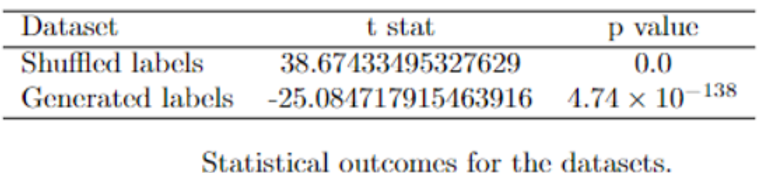
\includegraphics[width=8cm]{tstat.png}};
    \end{tikzpicture}
\end{figure}

We conduct a t-test between the inference probabilities for the correct outcomes, with and without knowledge for both datasets; both returning significant results suggesting that, at least statistically, both probability distributions are different and the embedded knowledge significantly changes the probability distribution for the correct outcome, this behavior can also be seen in the histograms for the probability distributions.

\begin{figure}[H]
    \centering
    \begin{tikzpicture}
        \node at (0,0) {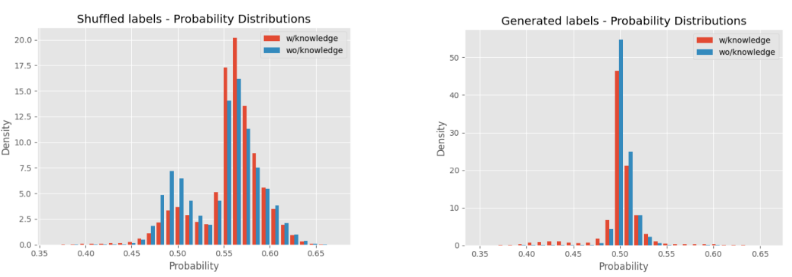
\includegraphics[width=8cm]{histogram.png}};
    \end{tikzpicture}
\end{figure}

The histogram for the synthetic dataset reflects the ambiguity of the model, with both distributions being concentrated at 0.5, whilst for the shuffled dataset the probabilities reach higher thresholds and the knowledge integration makes its distribution a little denser around higher probabilities.

\subsection{Triples}
Triples are dependency representations of sentences. For example, take the sentence ``David noticed he had put on a lot of weight recently'', using Spacy, we can generate triples, most commonly Subject-Verb-Object (SVOs), to represent the sentence with the most relevant context and information. Drawing inspiration from Aglinoby and Teugel (2022), where graph representations of possible answers to questions are used to determine the highest-ranking answer, our model will use extracted triples from the sentences comprising a story to compute a cosine similarity between the triples and two possible endings. Due to time limitations, the extracted triples we captured were done using speech tagging identification. Further refinement and possible improvement on triple extraction are discussed in the Conclusion.

\begin{figure}[H]
    \centering
    \begin{tikzpicture}
        \node at (0,0) {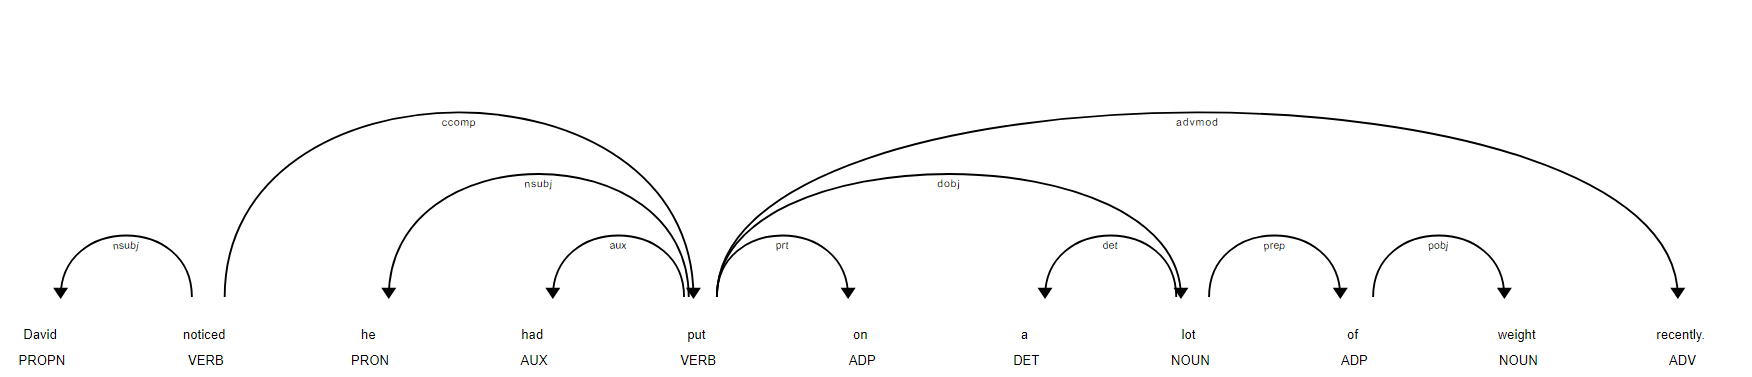
\includegraphics[width=8cm]{spacy.png}};
    \end{tikzpicture}
    \caption{Spacy Dependency Example}
\end{figure}

Using SPACY, we parse through all our sentences capturing words that are labeled ``ROOT" (for verb), ``nsubj" (for subject), or ``dobj"/``pobj" (for object) into our SVO triples. It is important to note that ``ROOT" can be a successful tag for verbs but isn't a guarantee. As noted in Figure 1, certain words 
such as ``put" are stronger central nodes than others since they share more dependencies.  This will be important to improve upon to capture significant SVOs optimally.

For our inference model, after generating SVOs, one for each story sentence, we use a Bert model to generate cosine similarities for our different endings. We accomplish this by tokenizing our SVOs; then, we run the tokenization through a Bert model to obtain a mean pooled output for each triple. The story endings are processed similarly. Next, we compute a cosine similarity between all the story sentences and the two possible endings (Figure 2).

\begin{figure}[H]
    \centering
    \begin{tikzpicture}
        \node at (0,0) {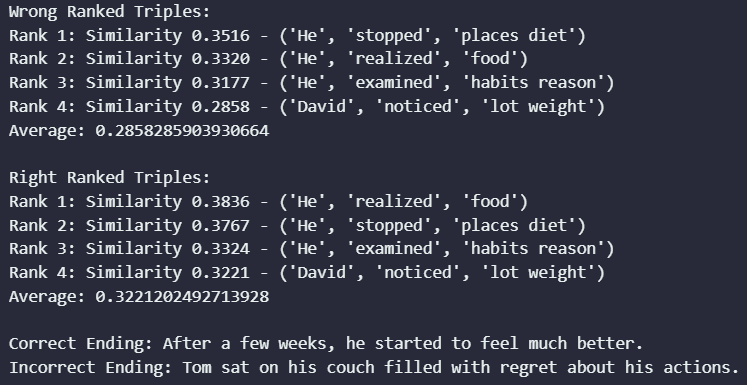
\includegraphics[width=8cm]{Cosine_Similarity.png}};
    \end{tikzpicture}
    \caption{Consine Similarity}
\end{figure}

In the figure above, we can see how the sentence we parsed in Figure 1, the associated triple is (David, noticed, lot weight), compares to the right and wrong endings. The average of all 4 triples' similarity to each story ending is used to determine the correct ending. We average the scores and predict the “correct” ending by selecting the max. In Figure 2, we would have correctly predicted the right ending since the average, 0.3221, was higher. Important to note, that for our approach we did not triple the story ending. We had concerns of possibly over-indexing on single sentence’s triple if they shared commonalities. By having all of the story’s ending instead, we believe to have mollified that concern.

In addition to the inference model, we used the BertForSequenceClassification configuration to train a model that used triples to predict the correct story ending.

Both approaches were used on the two versions of our dataset, GPT-generated story endings and mixed story endings. 

\section{Results}

\begin{figure}[H]
    \centering
    \begin{tikzpicture}
        \node at (0,0) {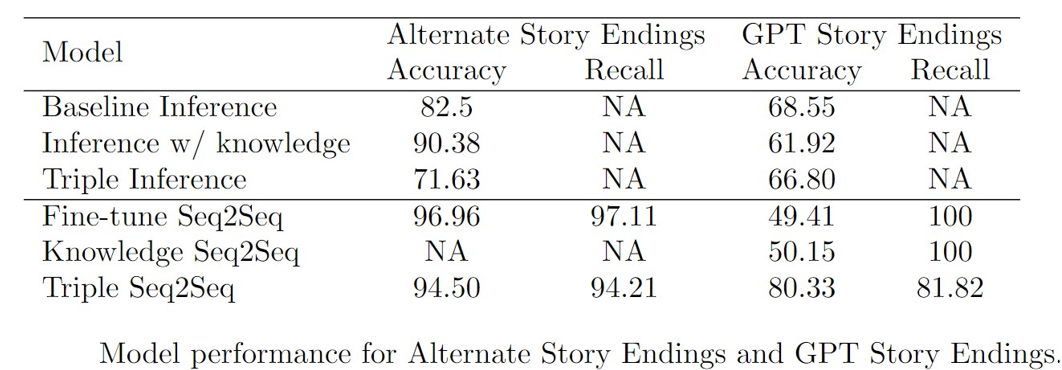
\includegraphics[width=8cm]{results.png}};
    \end{tikzpicture}
\end{figure}

\subsection{Accuracy Between Different Endings}
Our initial exploration with alternate story endings helped us level-set the task. The baseline model performed well at predicting the correct story ending, but the knowledge prompt approach resulted in the highest benchmark at inference. Suggesting that when the candidate outcomes are dissimilar enough, the additional knowledge increases the model’s performance. At this stage, we learned that the initial development of alternative endings that had little to no resemblance to the original story was too easy for the model. Here we decided to elevate the difficulty by creating GPT-generated story endings that shared more resemblance to the story’s subject matter. At inference, no approach was able to surpass the baseline for the synthetic dataset. Looking at the accuracies we see that the additional knowledge confuses the model more, sitting at 61.92\% accuracy. The triple method, sitting at 66.8\% and closer to baseline, is likely not complex enough to capture the stories’ most relevant aspects to surpass the dataset’s ambiguity without training. When fine-tuning the Seq2Seq model with the discussed methods, none can surpass fine-tuning the model with the raw alternate story-ending dataset.  However, the same model with the synthetic endings struggled to predict the correct classification, almost a coin flip. It’s here where we saw substantial improvements in the Triple approach, which proved to be the most successful. Condensing stories to core elements and relating them to the story’s ending helped augment the performance of the fine-tuned sequence classification model.

\subsection{Recall}
We encountered an issue with some of our models where Bert would return either 100\% or 0\% recall. This problem became apparent when the model was tasked with closely related endings: it would either predict all correct labels or all incorrect labels, failing to find a middle ground. 

\subsection{Data Challenges}
As mentioned earlier, our initial challenge was that the training dataset lacked incorrect endings and the testing dataset lacked labels. To address this, we generated incorrect endings by shuffling the correct labels randomly. However, this approach proved too simplistic for Bert to solve. To introduce a greater challenge, we utilized GPT-generated labels, ensuring a more complex problem for Bert to tackle. 

Another inherent challenge was that the sentences within the provided dataset varied widely in topic, length, complexity, and narrative style, posing difficulties for the model in identifying patterns. To expand our training dataset, we split each input into two versions: one with the correct ending and another with the incorrect ending. This effectively doubled the dataset's size, providing Bert with more diverse examples to learn from. However, this expansion also intensified the computational demands of fine-tuning a Bert model.

\section{Conclusion}

This project demonstrates the capability of enhancing common-sense reasoning tasks by augmenting the quality of inputs as opposed to scaling the model. We augmented our baseline by engineering knowledge prompts and extracting triples for our stories. In the future, we’d like to explore the benefits of combining both approaches to study any possible enhancements. Unfortunately, due to time constraints and resource limitations (Google Colab timeouts), we were unable to investigate that thread further.

Furthermore, another technique that we’d like to explore refining is triple extraction. As reported in the results, sequence classification worked best when paired with the triples method. However, for our project, the triple extraction method was only meant to start the inquiry process. All triples that were extracted were done so with the help of speech tagging. With more work and time, we can explore different methods and algorithms to capture stronger triples that better represent the sentences they come from. As mentioned previously, assumptions such as ROOT representing the verb were made - approaches like this could be further explored. Additionally, proper graphing techniques can be applied between the story’s sentences and the endings. 
The way the contextual knowledge is created could be improved as well to generate more relevant information about the stories, querying different models or procuring a more concise context could further improve the performance.

Also, while we’re confident in our approaches and the dataset we used to work with future studies should be replicated with different datasets that are verified and studied. The alternate story endings were not nuanced enough as demonstrated by the performance of the baseline model. While the GPT-generated story endings proved more challenging, for reproducibility and external generalization a dataset with predefined labels should be used for binary classification.

Lastly, these approaches can be further investigated and applied to domains. Any domain that is hampered by access, resources, or data can leverage the methods we have explored to retrieve the most insights. By acknowledging the limitations and areas for improvement in our current methods, and by exploring avenues for refinement and broader applicability, we can pave the way for more robust and insightful approaches to common-sense reasoning tasks in the future.


\begin{thebibliography}{999}
    \bibitem{Aglinoby}
    Aglionby and Teufel,
    \emph{Identifying relevant common sense information in knowledge graph}.
    aclanthology.org/2022.csrr-1.1,
    2022.

    \bibitem{Liu}
    Liu et al.,
    \emph{Generated Knowledge Prompting for Commonsense Reasoning}.
    aclanthology .org/2022.acl-long.225,
    2022.

    \bibitem{Mostafazadeh}
    Mostafazadeh et al.,
    \emph{LSDSem 2017 Shared Task: The Story Cloze Test}.
    aclanthology.org/ W17-0906,
    2017.

    \bibitem{Radford}
    Radford et al.,
    \emph{Improving Language Understanding by Generative Pre-Training}.
    2018.


\end{thebibliography}

\end{multicols}

\end{document}

